\documentclass[12pt,a4paper,oneside]{article}
\usepackage[colorlinks=true]{hyperref}
\usepackage[utf8]{inputenc}
\usepackage[czech]{babel}
\usepackage{pdfpages}
\usepackage{graphicx}
\textwidth 16cm \textheight 25cm
\topmargin -1.3cm 
\oddsidemargin 0cm
\usepackage{footnote}
\pagestyle{empty}
\begin{document}
\title{Modul převodníku TTLRS48501A}
\author{Jakub Kákona, kaklik@mlab.cz}
\maketitle

\thispagestyle{empty}
\begin{abstract}
Modul je určen pro připojení procesorových modulů na sběrnici RS485.
\end{abstract}

\begin{figure} [htbp]
\begin{center}
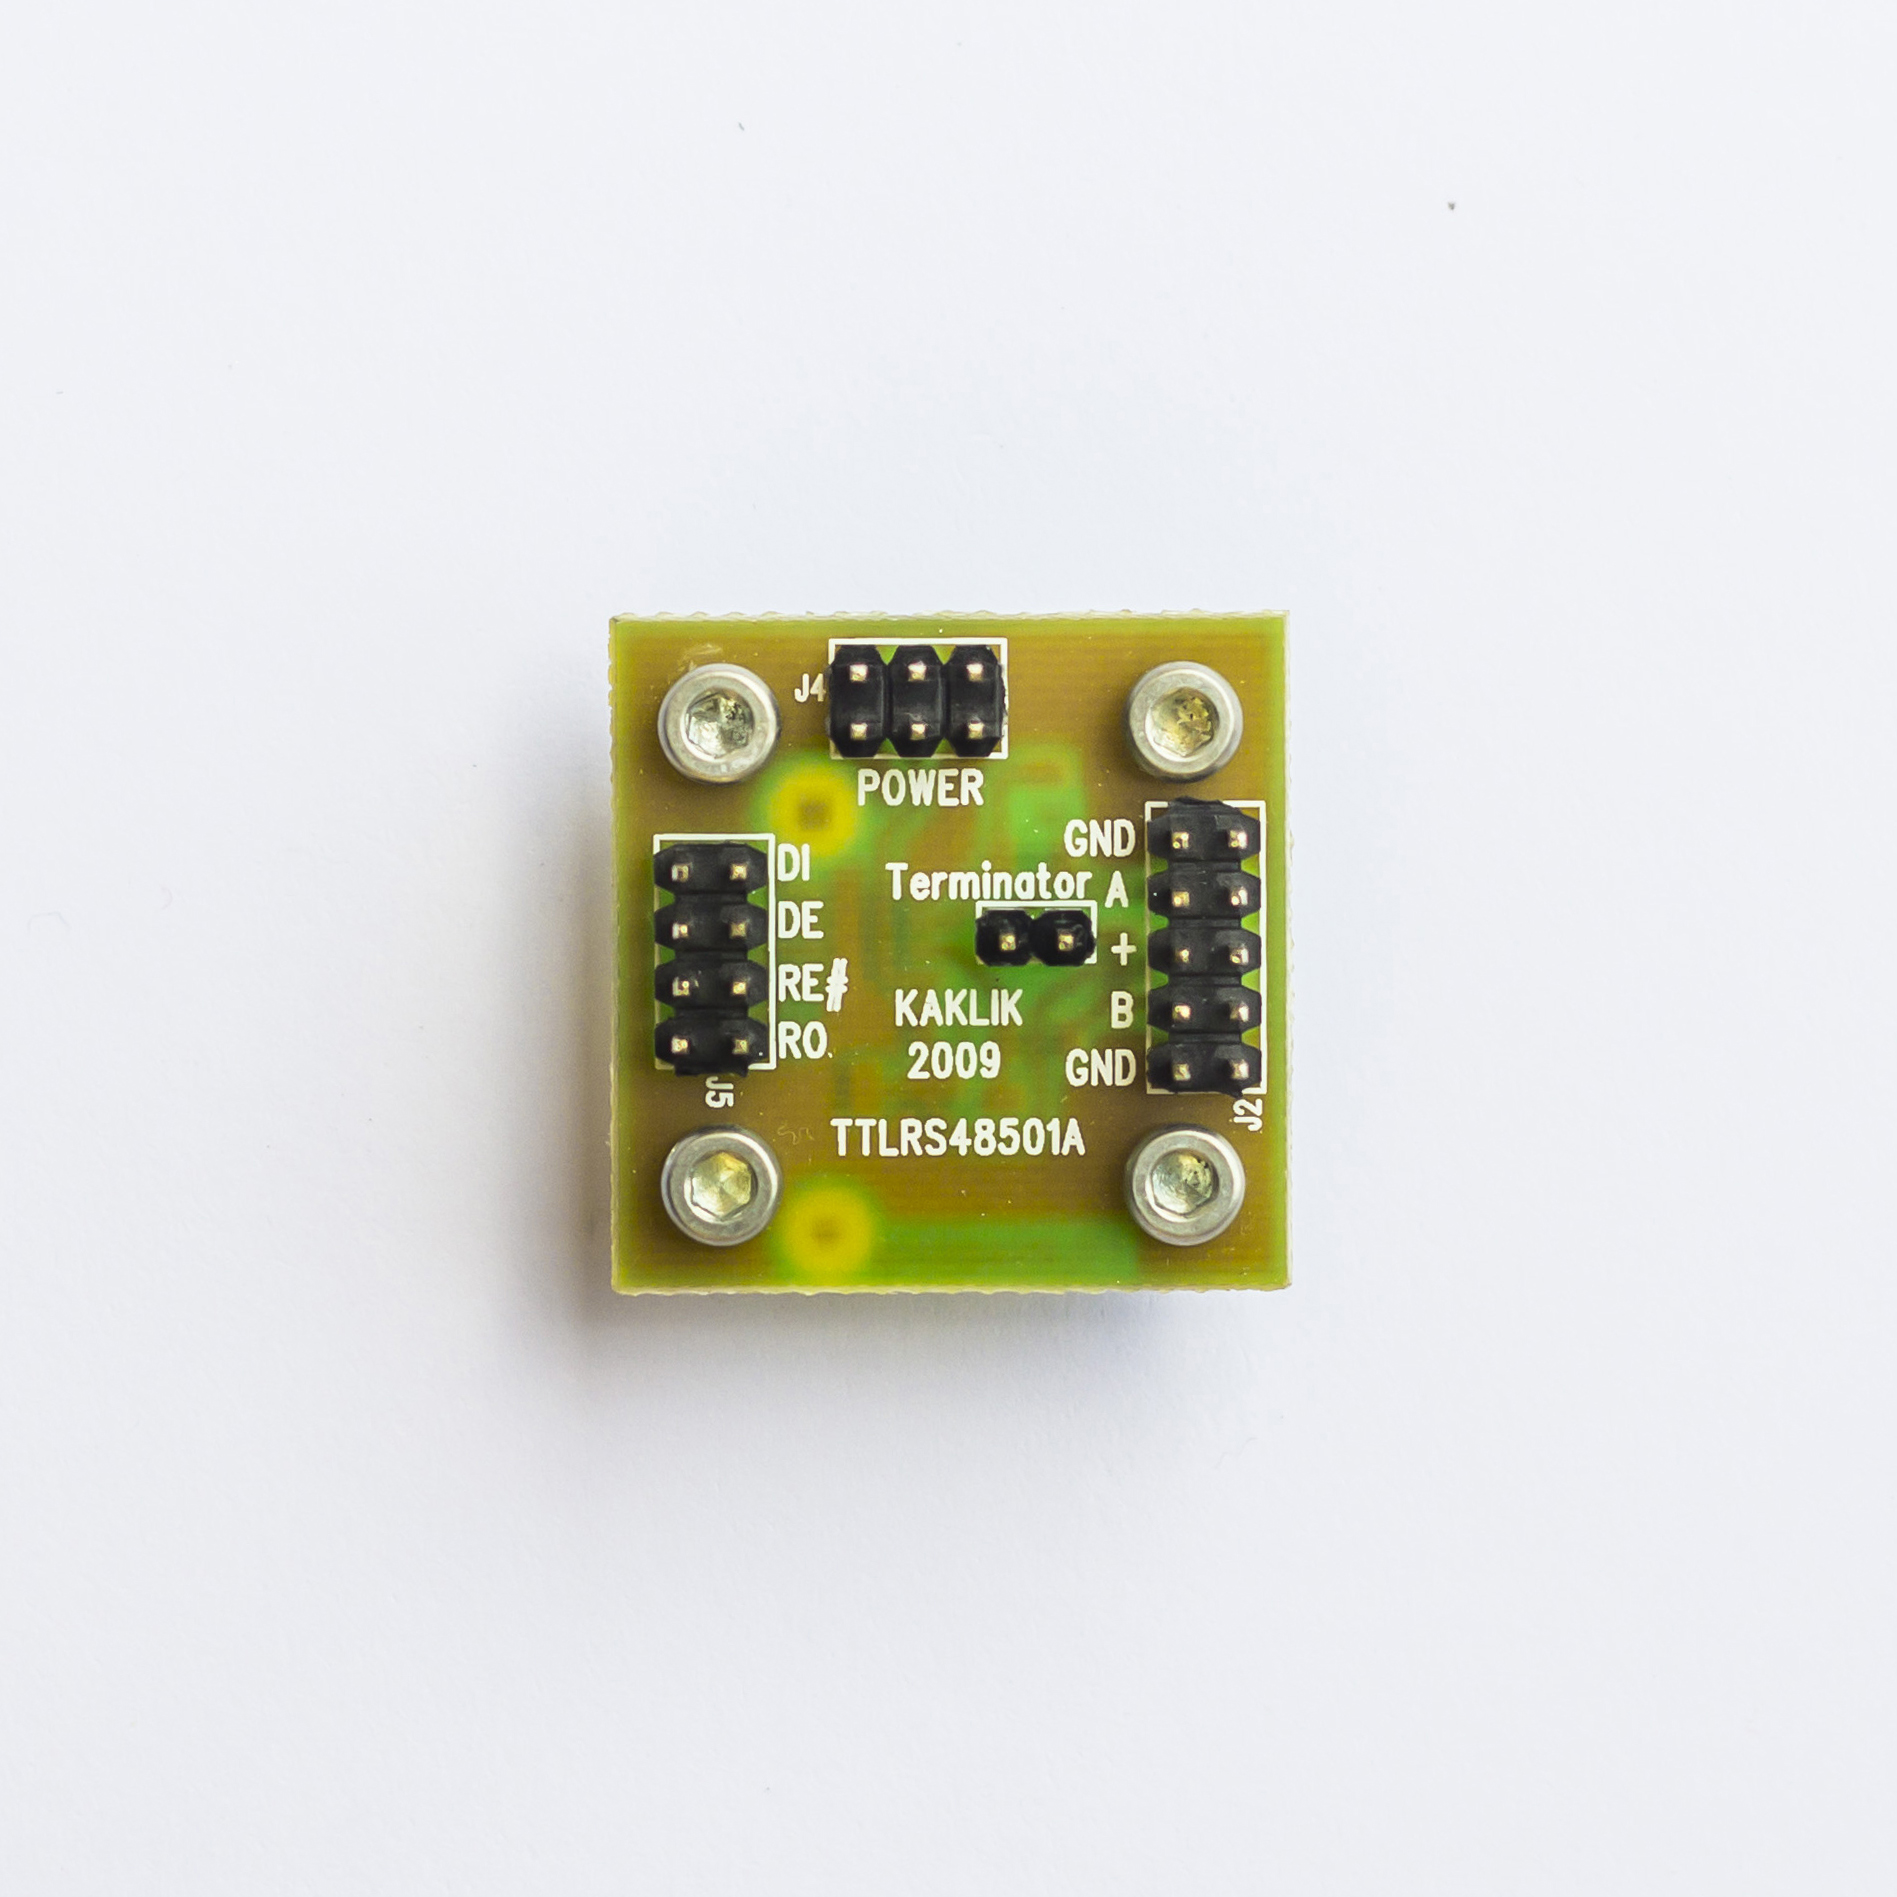
\includegraphics [width=80mm] {./img/TTLRS48501A_Top_Big.JPG} 
\end{center}
\end{figure}

\begin{figure} [b]

\includegraphics [width=25mm] {./img/TTLRS48501A_QRcode.png} 
\end{figure}

\newpage
\tableofcontents


\section{Technické parametry}
\begin{table}[htbp]
\begin{center}
\begin{tabular}{|c|c|c|}
\hline
\multicolumn{1}{|c|}{Parametr} & \multicolumn{1}{|c|}{Hodnota} & \multicolumn{1}{|c|}{Poznámka} \\ \hline
Napájecí napětí & +5V &  30 mA \\ \hline
Pracovní napětí  vstupů & do $\pm$ 10V &  \\ \hline
Maximální budící proud výstupů & 60 mA & \\ \hline
\end{tabular}
\end{center}
\end{table}

\newpage
\section{Popis konstrukce}

\subsection{Zapojení}
Modul obsahuje základní ochranu proti přepěťovým špičkám a terminační rezistor který lze juperem odpojit, což je výhodné pro moduly, které jsou zapojeny uprostřed sběrnice.  Datové vývody  jsou vyvedeny na hřebínky ve standardní konfiguraci MLAB, která je vhodná pro kratší mezimodulové spoje. V případě potřeby použití modulu na delší spoj (desítky metrů) je vhodné k modulu přidat ochranné transily pro zvýšení odolnosti proti přepětí. To lze udělat připojením konverzního modulu s konektorem RJ45. Pak lze použít standardní UTP patch kabely, které jsou vhodné pro vedení na delší vzdálenosti.   

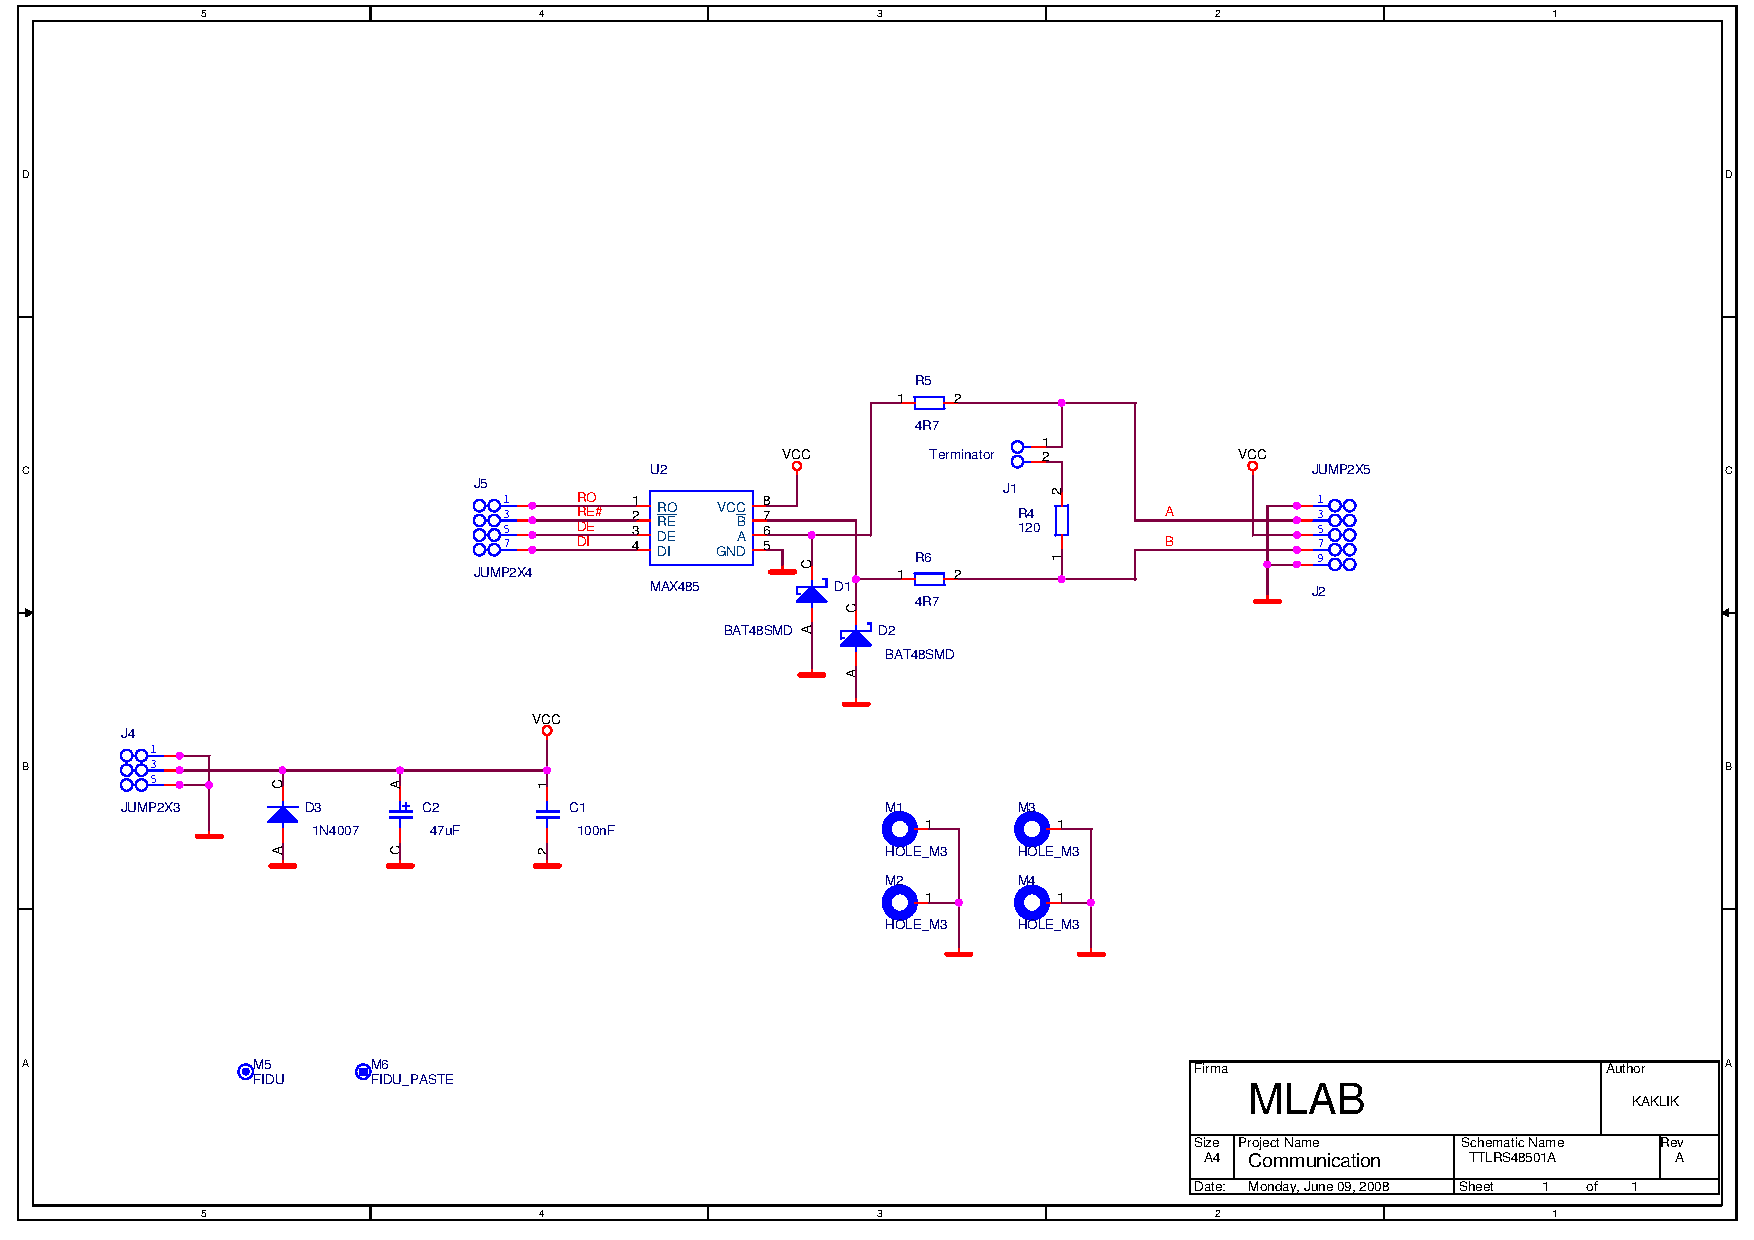
\includepdf[pages={1},landscape=true]{../../SCH/TTLRS48501A.pdf}

\subsection{Odrušení}

Vyzařování je v případě modulu značně potlačeno  differenční fyzickou vrstvou sběrnice.  K její správné funkci je ale potřeba využívat kroucených párů.  Pro vedení signálů RS485 jsou proto vhodné například UTP kabely.  

\section{Výroba a testování}

Modul se testuje optickou kontrolou spojů a následným připojením na laboratorní zdroj s omezením proudu. Dále by po připojení dvou modulů k USBRS23201B a nastavení jednoho modulu na příjem a druhý na vysílání mělo být možné posílat znaky. Podrobněji je tento testovací postup popsán na wiki \cite{wiki-TTLRS48501A}.


\subsubsection{Osazení}

Modul se osazuje standardním způsobem požívaným pro SMD součástky. 

\begin{figure} [h!tbp]
  \centering
  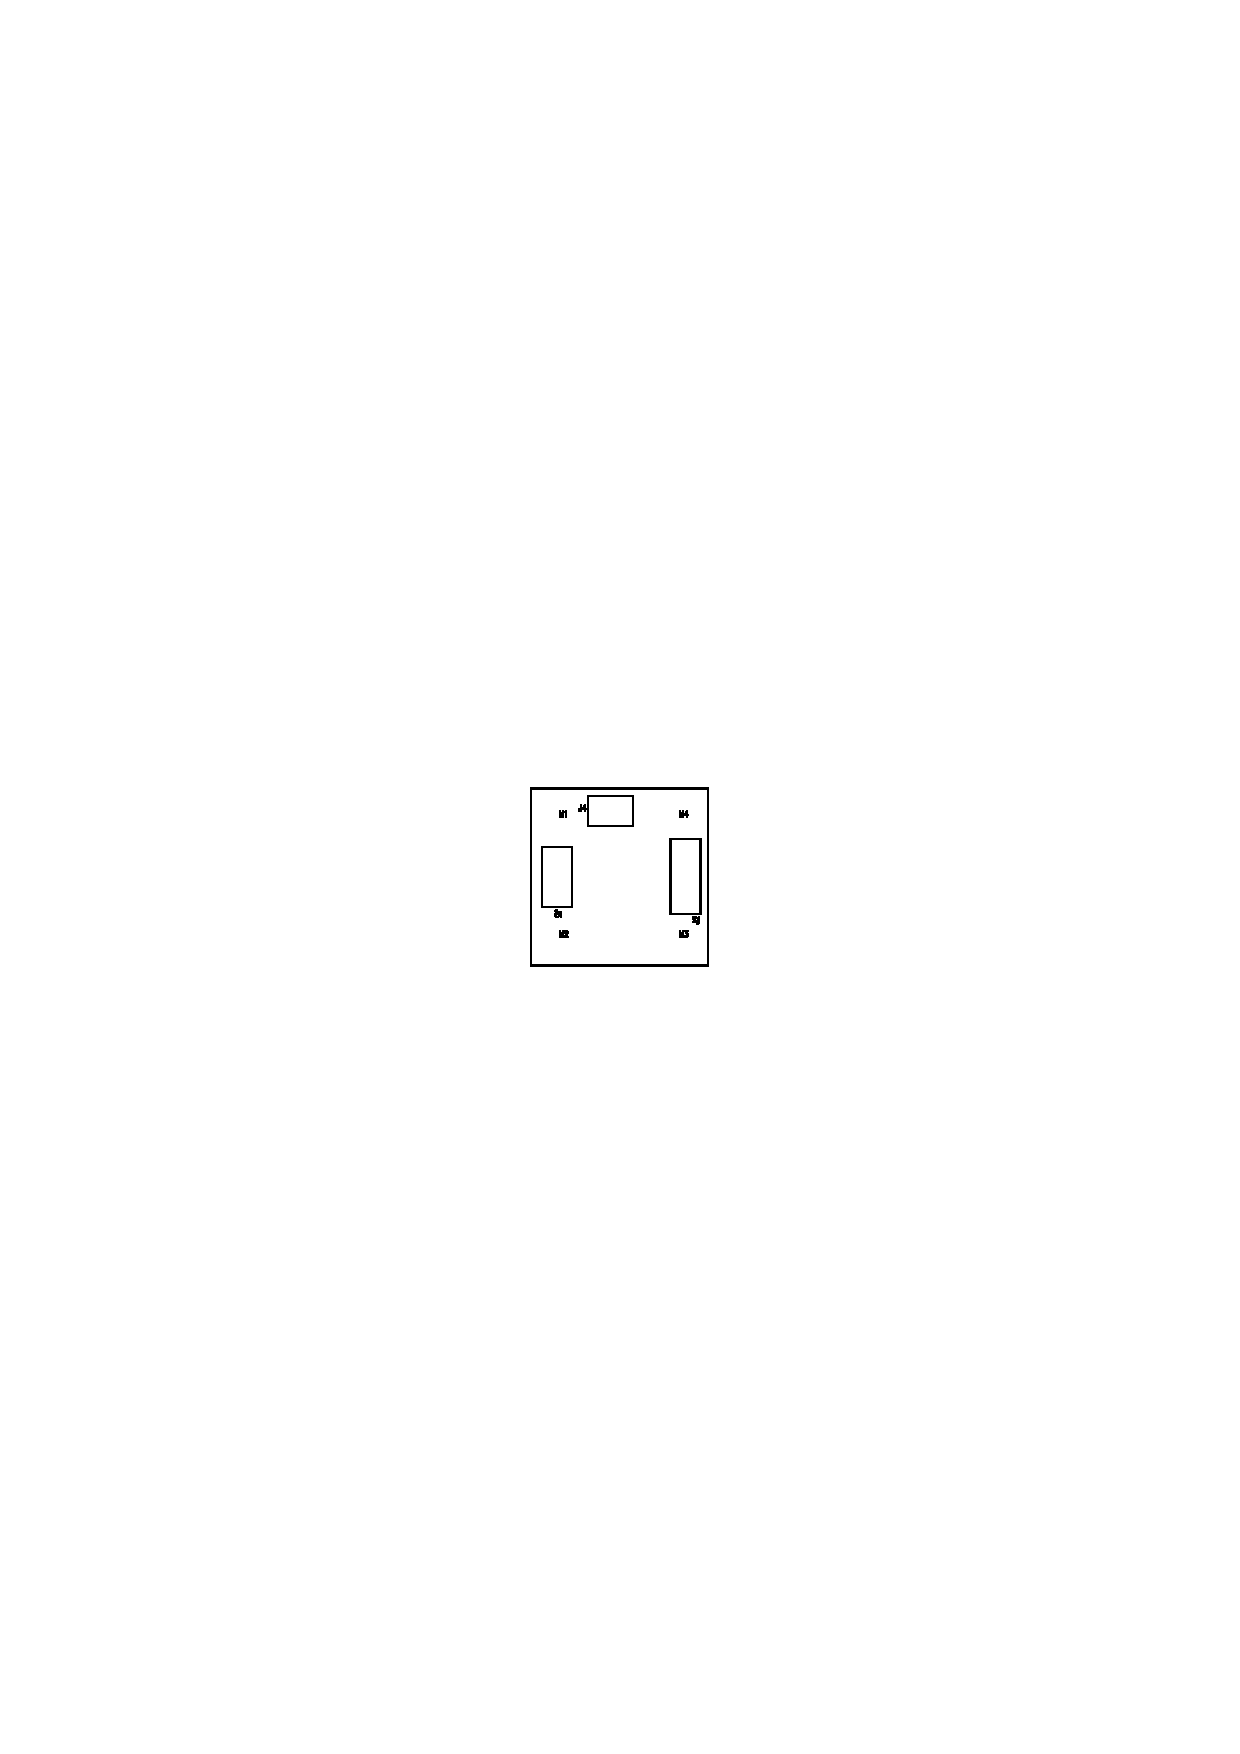
\includegraphics[trim = 8.5cm 13.0cm 8.5cm 13.0cm, clip, width=6.5cm]{../../CAM_DOC/O1.pdf}
  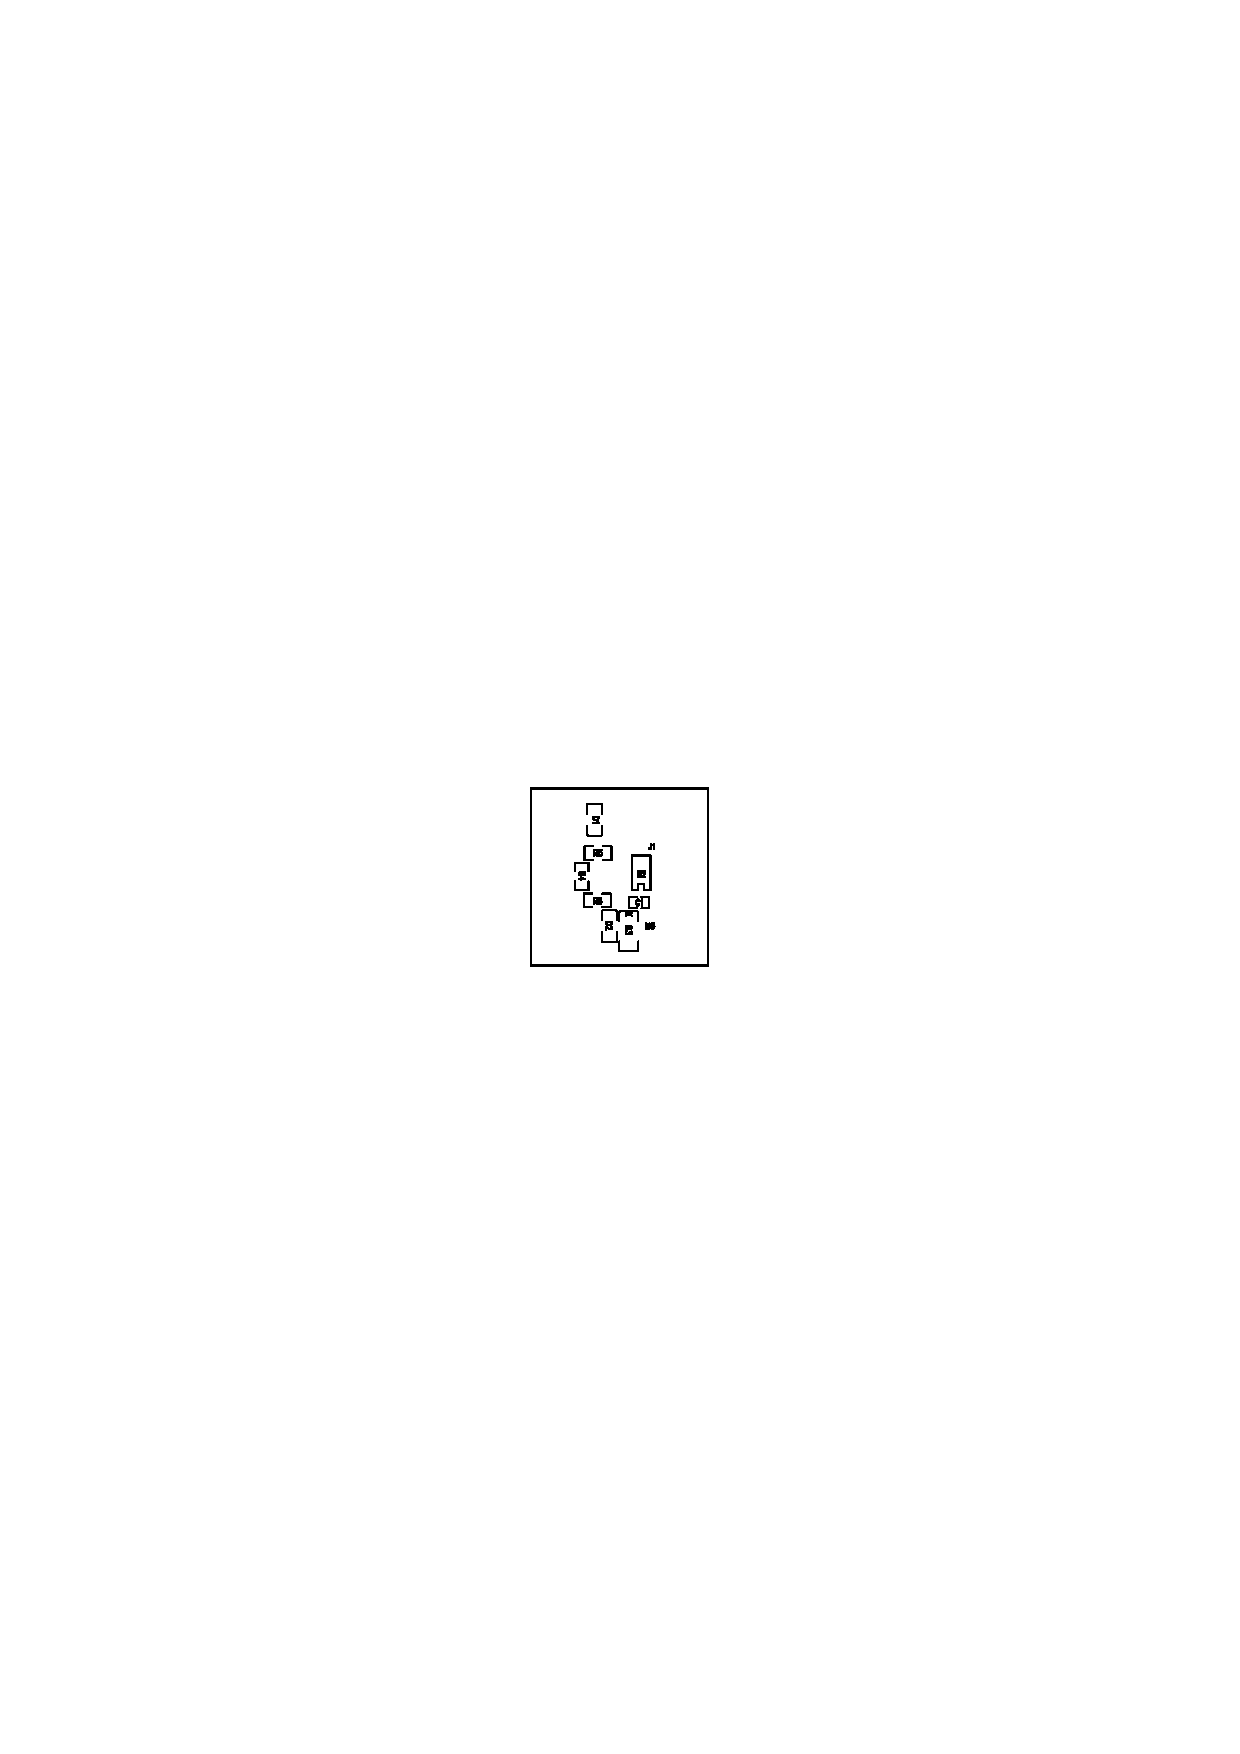
\includegraphics[trim = 8.5cm 13.0cm 8.5cm 13.0cm, clip, width=6.5cm]{../../CAM_DOC/O2.pdf}
  \caption{Osazovací plán horní a spodní strany plošného spoje}
  \label{fig:osazovaci_plan}
\end{figure}

\begin{savenotes}
\begin{table}[h!]
\begin{center}
\begin{tabular}{ |c|c|c|c| }
\hline 
Počet & Označení & Typ  & Pouzdro  \\ 
\hline 
1	&	C1	&	100nF	&	C0805	\\
1	&	C2	&	47uF	&	ELYTB	\\
2	&	D1,D2	&	P4SMA15A	&	SMB	\\
1	&	D3	&	M4	&	SMA	\\
1	&	J1	&	Terminator	&	JUMP2	\\
1	&	J2	&	JUMP2X5	&	JUMP2X5	\\
1	&	J4	&	JUMP2X3	&	JUMP2X3	\\
1	&	J5	&	JUMP2X4	&	JUMP2X4	\\
1	&	R4	&	120	&	R1206	\\
2	&	R5,R6	&	10R	&	R1206	\\
1	&	U2	&	MAX485	&	SO8\_150	\\
\hline 
\end{tabular}
\end{center}
\caption{Seznam součástek osazovaných na desku plošného spoje.}
\label{seznam_soucastek_galvanic_isolation}
\end{table}
\end{savenotes}



\section{Programové vybavení}

Samotný modul pro svoje  fungování nepotřebuje speciální firmware. Potřebuje však pro svojí správnou funkci pin řídící směr toku dat.  

\begin{thebibliography}{99}
\bibitem{wiki-TTLRS48501A}{TTLRS48501A MLAB wiki} 
\href{http://wiki.mlab.cz/doku.php?id=cs:ttlrs485}{Převodník úrovní TTL a RS485 TTLRS48501A}

\end{thebibliography}
\end{document}